\section{Algorithme d'affectation}
\label{sec::moulinette}

\begin{figure}[H]
	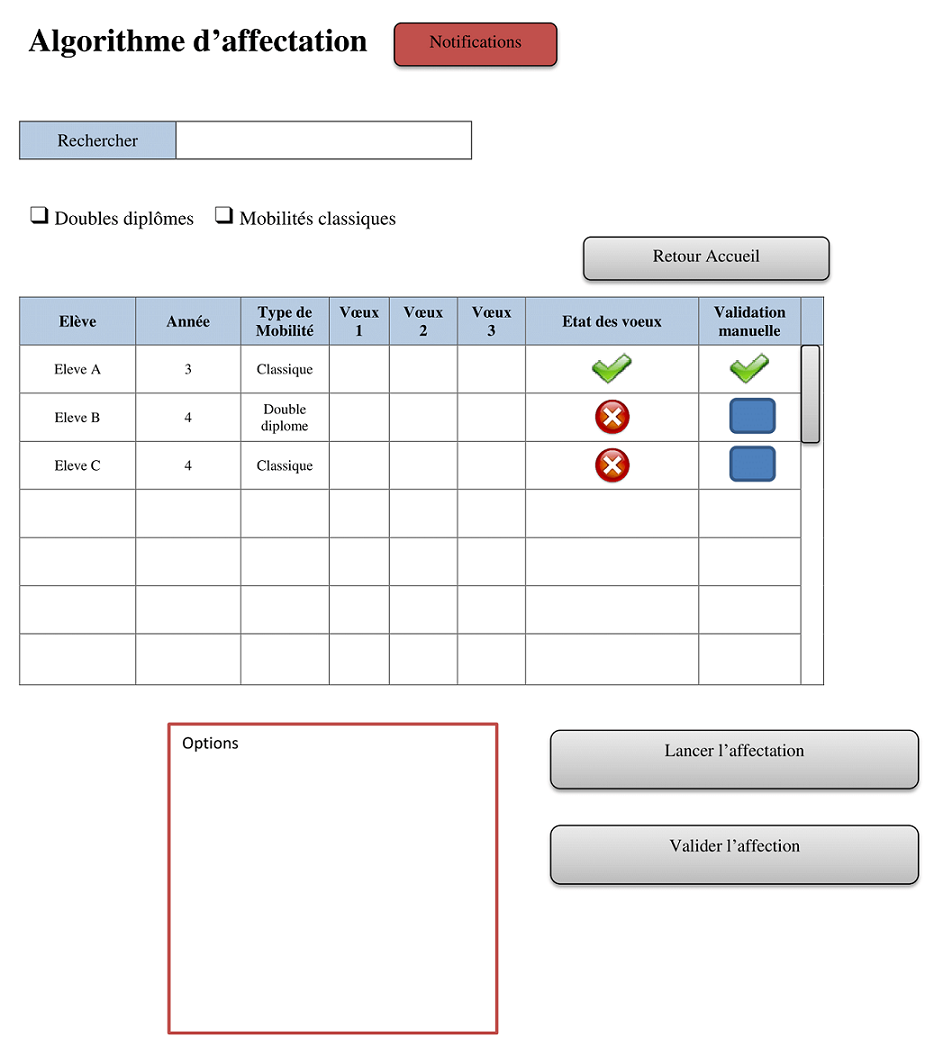
\includegraphics[scale=0.7]{Admin/Moul.png}
	\caption{Page de gestion de l'algorithme d'affectation}
	\label{fig::moulinette}
\end{figure}

La figure \ref{fig::moulinette} présente la page sur laquelle se trouve un tableau récapitulant les vœux définitifs des élèves, après la fin des choix de vœux (phase 1). Ce tableau comprend donc la liste des élèves, leur année, la liste des vœux, le type de mobilité choisie (double diplôme, mobilité classique), leur état (validé, à validé).

Encore présent sur ce tableau; une zone de recherche par mot clé ainsi que plusieurs filtres (années, universités, type de mobilité...).

\bigbreak

L'administrateur peut, sur cette page, gérer les paramètres de l'algorithme avant de le lancer (ajout de paramètres particuliers modifiant l'ordre d'attribution des vœux, en plus des notes).

\bigbreak

Il est aussi possible à l'administrateur de valider les vœux d'un élève manuellement. Cela fait sortir cet élève de la liste des élèves concernés par l'algorithme (il apparaitra toujours dans la liste des élèves mais son état deviendra "validé" et il ne sera pas pris en compte par l'algorithme).

\bigbreak

En bas de la page, deux boutons sont présent. Le premier, "Lancer l'algorithme" permet d'affecter les vœux aux élèves suivant les options choisies. Suite au lancement de cet algorithme, l'administrateur peut, si il le désire invalider l'affectation afin de modifier les options et lancer une nouvelle session d'affectation. Après la validation de l'affectation, il est toujours possible à l'administrateur de modifier les vœux des élèves manuellement.

\bigbreak

Le deuxième bouton valide l'affection et déclenche le passage à la phase numéro 2. Cette action, met à jour les vues des élèves et de l'administrateur qui auront par la suite accès à l'interface de la phase 2, à savoir, la gestion des documents pour la préparation de la mobilité. 